\documentclass[aspectratio=169]{beamer}
\usetheme[block=fill]{metropolis}
\usepackage{tikz}
\usetikzlibrary{shapes.geometric, arrows.meta, positioning, calc}

\title{Building a Reproducible Scholarly Search Toolkit}
\subtitle{Episode 2: Clean-Room Package Architecture}
\author{Scholar Search Kit}
\date{}

\begin{document}

\begin{frame}[plain]
  \titlepage
\end{frame}

\begin{frame}{Episode Goal}
  \begin{alertblock}{The Goal}
    Set up a professional, extensible Python package architecture using \texttt{uv} and \texttt{pyproject.toml}.
  \end{alertblock}
  \vspace{0.5cm}
  We will establish a strict folder structure that enforces our component boundaries and prevents cyclic imports before writing a single line of application logic.
\end{frame}

\begin{frame}{The Project Layout}
  \begin{center}
  \resizebox{0.7\linewidth}{!}{
  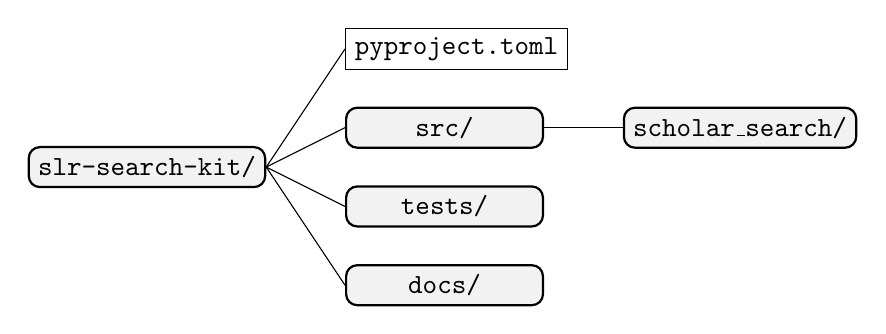
\begin{tikzpicture}[
      node distance=0.5cm and 1cm,
      folder/.style={rectangle, draw, thick, rounded corners, minimum width=2.5cm, fill=black!5, align=left},
      file/.style={rectangle, draw, minimum width=2.5cm, align=left}
    ]
    
    \node[folder] (root) {\texttt{slr-search-kit/}};
    
    \node[file, right=of root, yshift=1.5cm] (pyproject) {\texttt{pyproject.toml}};
    \node[folder, right=of root, yshift=0.5cm] (src) {\texttt{src/}};
    \node[folder, right=of src] (pkg) {\texttt{scholar\_search/}};
    \node[folder, right=of root, yshift=-0.5cm] (tests) {\texttt{tests/}};
    \node[folder, right=of root, yshift=-1.5cm] (docs) {\texttt{docs/}};

    \draw[-] (root.east) -- (pyproject.west);
    \draw[-] (root.east) -- (src.west);
    \draw[-] (root.east) -- (tests.west);
    \draw[-] (root.east) -- (docs.west);
    \draw[-] (src.east) -- (pkg.west);
  \end{tikzpicture}
  }
  \end{center}
\end{frame}

\begin{frame}{Dependency Management with \texttt{uv}}
  \begin{block}{Why \texttt{uv}?}
    A blazingly fast package manager written in Rust. It replaces \texttt{pip}, \texttt{venv}, and \texttt{pip-tools} with a single, highly reproducible interface.
  \end{block}

  \begin{itemize}
      \item \texttt{uv init}: Scaffolds the project.
      \item \texttt{uv add}: Pin dependencies reliably.
      \item \texttt{uv sync}: Ensures the environment exactly matches the lockfile.
  \end{itemize}
\end{frame}

\begin{frame}{Implementation: `pyproject.toml`}
  \begin{block}{The Manifest}
    Defines the package metadata, entry points, and dependencies.
  \end{block}
  
  Key configurations:
  \begin{itemize}
      \item \texttt{[project]}: Name, version, requires-python.
      \item \texttt{[project.scripts]}: Binds the CLI to \texttt{scholar-search}.
      \item \texttt{[tool.pytest.ini\_options]}: Configures the test runner to use the \texttt{src} layout.
  \end{itemize}
\end{frame}

\begin{frame}{Verification}
  \begin{alertblock}{Success Criteria}
    \begin{itemize}
        \item The project installs cleanly with \texttt{uv sync}.
        \item Tests run successfully via \texttt{pytest}.
        \item No cyclic import warnings.
    \end{itemize}
  \end{alertblock}
\end{frame}

\end{document}
